\section{Ejercicio 7}
\subsection{Desarrollo}
Analizamos con varios grupos de tareas el comportamiento de $SchedMistery$ para llegar a los siguientes resultados:

\begin{enumerate}[(a)]

\item El scheduler $SchedMistery$ es un RoundRobin modificado

\item La modificación se da en el tiempo que se le permite correr a cada tarea antes de ser desalojada

\item Dicha modificación tiene en cuenta dos cosas: los parámetros de entrada del programa y si quedan otras tareas que pueden correr.

\item Si no hay otras tareas que puedan correr no hay desalojo, la tarea Idle sólo aparece cuando no hay tareas que puedan correr.

\item En cuanto a los tiempos de ejecución de cada tarea, la primera aparición de la tarea es de un tick de reloj, mientras que el resto equivale al valor de la entrada, tomada secuencialmente (explicado más abajo con los gráficos)

\item Las ejecuciones de las tareas fuera de los tiempos dados en la entrada del programa son iguales a la última corrida correspondiente a los valores de la entrada.

\item De no haber otras tareas que puedan ejecutarse, se siguen contando los valores de los parámetros de entrada

\end{enumerate}

\subsection{Experimentación}

Ahora mostraremos de donde obtuvimos la información antes mencionada

Los lotes utilizados fueron:\\

loteEj7a.tsk\\
TaskCPU 18\\
TaskCPU 18\\
TaskCPU 18\\
TaskCPU 18\\


loteEj7b.tsk\\
\#Tarea intensiva de CPU 1\\
TaskCPU 18\\
\#Tarea intensiva de CPU 2\\
@7:\\
TaskCPU 20\\
\#Tarea interactiva 1\\
TaskConsola 4 3 6\\
\#Tarea interactiva 2\\
TaskConsola 8 2 7 \\





\begin{figure}[H]
  \centering
    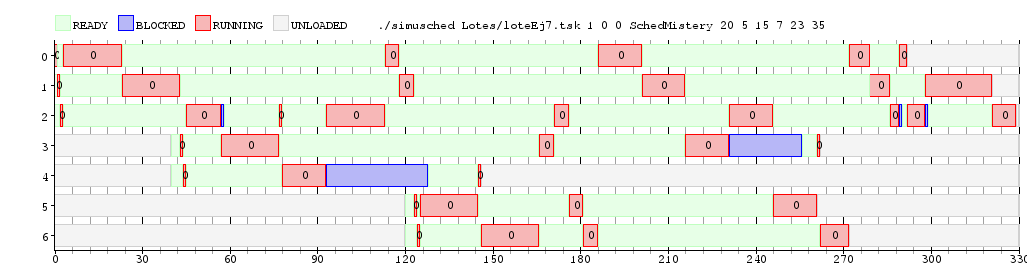
\includegraphics[width=1.1\textwidth]{imagenes/test1ej7.png}
  \caption{Se pueden apreciar (a)(b)(e)(f)}
  \label{fig:ej7a}
\end{figure}

En esta figura se puede ver claramente que es un Round Robin y que los tiempos que toman las tareas cada vez que entran en Ready son 1, 3, 2, 4, 4.. Luego de la cuarta vez que el scheduller pone a correr la tarea, siempre le da 4 tics de reloj


\begin{figure}[H]
  \centering
    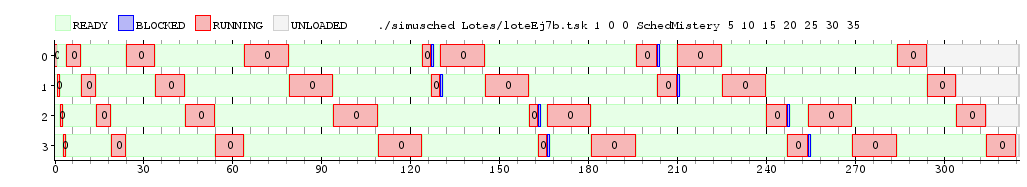
\includegraphics[width=1.1\textwidth]{imagenes/test2ej7.png}
  \caption{Se pueden apreciar (a)(b)(d)}
  \label{fig:test2ej7}
\end{figure}


\begin{figure}[H]
  \centering
    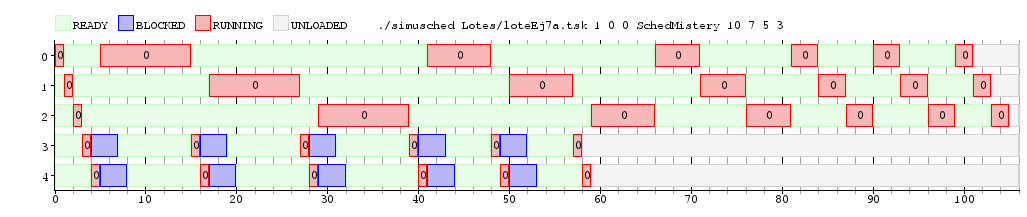
\includegraphics[width=1.1\textwidth]{imagenes/test3ej7.png}
  \caption{Se pueden apreciar (a)(b)(c)(e)(f)(g)}
  \label{fig:test3ej7}
\end{figure}
